\chapter{Novel learning theory}
Since the previous analysis of the learning model, we can then notice a few disadvantages and a few very subtle points that we omitted. It is apparent that the analysis is somewhat entangled, with various situations, interpretations, setting and assumptions together, and with a non-unified structure of models in question. The system in which the model is considered and analysed is also missing in essence. There are a lot of ambiguities around what is considered and what is not, even with probabilistic nature and the deterministic aspect. Terms like \textbf{latent spaces} and many do not capture the entire dynamic or meaning of the system. It is then we introduce our novel analytical framework, namely the \textbf{Unified Unitary Construct} framework. It is however, can be said otherwise that the learning theory is rather not so novel, but approaching the problem is a more distinct way of the already existing framework. 
\section{Motivation}
The predecessors of neural network, for operations and purposes, take in the form of a specific application of function constructs, finite singleton algorithms. For such purposes, a specific classical model $m$ takes the form of a single structure, with complex construction, often offering fixed architecture of its representation. Neural network is an attempt, for its philosophy, to change the aforementioned philosophy of constructing machine model by considering compute unit \cite{mcculloch_logical_1943,Rosenblatt1958ThePA}. 

Motivated by earlier analysis and observations, it is apparent that the analysis is entangled, with various situations, interpretations, setting and assumptions together, and with a non-unified structure of models in question. The system in which the model is considered and analyzed is also ineffective when considering larger structures or more `realistic' consideration aside from very simplified, strong system itself. There are a lot of ambiguities around what is considered and what is not, even with probabilistic nature and the deterministic aspect. Terms like \textbf{latent spaces} and many do not capture the entire dynamic or meaning of the system. It is then we introduce our novel analytical framework, namely the \textbf{Unified Unitary Construct} framework. It is however, can be said otherwise that the learning theory is rather not so novel, but approaching the problem is a more distinct way of the already existing framework. 

Recalled the classical learning framework, for $h$. We know and construct the principle of the system by settle on $h:\mathcal{X}\to \mathcal{Y}$, for any arbitrary defined in-out 2-tuple. Hence, the overall construction of a given model can be abstracted into layers of responsive results. This in particular draws some advantages, for example, can be easily approximated or expressed in the black box model style, or empiricism approach. However, it also comes with the drawback that we have seen, in the sense that the interpretation of such black box model is very narrow, even after we add different kind of flavours, for example, the assumptions of the Gaussian noise. This is majorly because of applying and addition of different components without a general framework, leading to a lot of messiness when looking directly into the theory itself. Specifically, for example, is the fact that there exists two kinds of learning analysis, one considers the information-theoretic approach of information exchange, while the other is simply the classical approach given in such the intrinsic noise error given by the observation set itself, keeping the classical theory intact. How to formalise this is a big hurdle to incorporate each other in, without considering the wider framework - one of the main problem with the speciality of learning theory. Nevertheless, at least accordance to general theory of the current date, formalization in to unit-like processing unit as \textit{neural network components} is one thing that should be considered for the learning framework. This is also one of the main point for the word \textbf{Unified} in our theory. 

\section{Principle}

We are motivated from earlier analysis, further experimental results, and arguably practical observations of empirical-based architectures that we find interesting. Oddly enough, the idea is encouraged of the observation that \textit{deep neural network} organising architecture might be more general than it is, particularly in the sense of mathematical modelling and structural implicit approximation, as well as factors like scalability, generality, and else. Furthermore, one of the purpose of this novel theory is also to redefine the entire learning space to, at least if not entirely original, might as well fall into the category of a reformulation of theoretical framework and not partaking the role of replacing it. 

As such, we need some principles to get started the analysis. What can those be that guarantee the success of a particular reformulation at first? For starter, we indict on the requirement of developing a general framework of neural network-like organisation for our models, both in the interpretation of the learning objective, and the structure of the hypothesis learner. Secondly, we have to define learning as a barebone process, of which then we will have to justify \textit{probabilistic nature} of it and the degree in which that is true. Thereby, we will then also have to reconsider the learning problem, under what scope of the problem and the classes of learning that is there to be achieved, the encoding space and what it is meant to, and the criteria of guaranteeing such learning to be probable. For now, those are enough, but the development that come afterward will justify it instead of the principle. 

Indeed, we can see the principle here - we want to redefine learning process in an organized manner, with minimal messiness from considering all factors together, and normalize the interpretation of \textit{unit-wise} architecture that neural network uses up to more. 

\subsection{Planning}

Then, what is the plan? The goal is to \textit{systematically introduce} the concept and the novel theory. Hence, we will separate it into discrete small step size parts. First, we need to conform the setting with a new template. This mean the following order is needed. 
\begin{enumerate}[leftmargin=1cm,itemsep=2pt,topsep=2pt]
  \item Introduce and define the formalism of an \textit{ambiance space} and an \textit{encoding space}. Those two will come in together to form the majority of $S$ as per system dynamic notation. 
  \item In the \textit{collection} $S$ should we extend it further, there always exists the object $h$, belonging to certain configuration class $\mathcal{H}$. We need to define this particular object, and its interaction to the collection itself. Which means, the ambiance space and encoding space. How do we bring up the \textit{representation concept} here altogether? 
  \item To start the mechanics, we need the \textit{mechanical space} $M$ to be defined. What can be it? What connects and form the structural description that $S$ make with the ambiance space, encoding, representation, subject dynamics, and else? 
  \item Now, come to the \textit{operational process}. For this, let's assume we have two different systems, in accordances, $S_{1}$ and $S_{2}$, each of which houses $h$, and $c$ respectively. How do they communicate? How, should it be done, can the operational space indict particular objective, or requirement, such that $h$ is evaluated, and $c$ is evaluated? What is hidden of $h$, and what is hidden of $c$? 
  \item Then, finally, bounds, theorems, analytical results, algorithmic consideration and conjectures that fit, into this description. 
\end{enumerate}
From the scope of it, it might seem not too practical to call as novel. But as far as we are considered, there should be something to take account on, and we need to do them carefully, such is to say there has been none, of which partake in said direction. There is a reason why messy construction being the worst nightmare of any people using the house, and we are the one to fix it, or at least attempted so. 

\section{System space}

The goal of the system space is to specify everything that contributes to the system dynamic. Or rather, any component, objects, subject structures, and so forth that acts, that exist, that is considered of interest in a given context. The principle is simple, to separate between the \textit{assumed shape} of an object from it representation or encoding. This can be done by specifying two parts - the \textit{ambiance space}, of which contains all the object in consideration, minus their properties and so of, and the \textit{encoding space}, which as its name implies, encodes all relevant structural information and properties that is considered, of said object. Just consider the very simple example of a car, specifying the barebone existence of it in an operational space, and the encoding space of the specific details of such cars, and factors affecting such. 

Before doing anything, let us define what is meant by ambiance space, and subsequently, encoding space, via a more statement-form definition. First, let us define the \textit{system space}. 
\begin{definition}[System space, Preliminary version]
  For any `procedural' structures, objects, realization \footnote{In the sense of explicit construction like coding, creating models that will have to be evaluated, instead of mathematical static statements and of operational means.}, we define the \textit{system space} $\mathcal{S}$ as the space containing two types of facilities that support it, the \textit{ambiance space} for where objects are realized, and the \textit{encoding space} where their realization is encoded and supported of its operation. 
\end{definition}

Hence, in essence, the system space includes, and contain the realization of the object itself. Such object can be anything, apple, baskets, logical system, interpretable text structure, 'unstructured data' in a sense, and so on. The accompanying space of the system space, however, is the encoding space. 

\begin{definition}[Encoding space, Preliminary version]
    The encoding space $\mathcal{E}$ of particular system space $\mathcal{S}$, contains the information and structural encoding of objects of the ambiance space $\mathcal{A}$, within certain representation scheme. 
\end{definition}

The ambiance space is simply defined as followed, of which contains the ambiance of the system. 

\begin{definition}[Ambiance space, Preliminary version]
    The ambiance space $\mathcal{A}$ is defined as the collection of objects of interest, with minimal observational language specifying it, and contain the raw, non-encoded subject of interest. 
\end{definition}

This contrast, even though we take inspiration from it, the ambiance space in the context of mathematical geometry and the like. For mathematics, the \textit{ambiance space} of a given object $x$ is the surrounding space of that mathematical object. So, if we study $\{x\}$, then its ambiance space is the $\mathbb{R}$ set. If $x$ is specified to be of high-dimension, then so on for $\mathbb{R}^n$. 

\begin{figure}[htb]
  \centering
  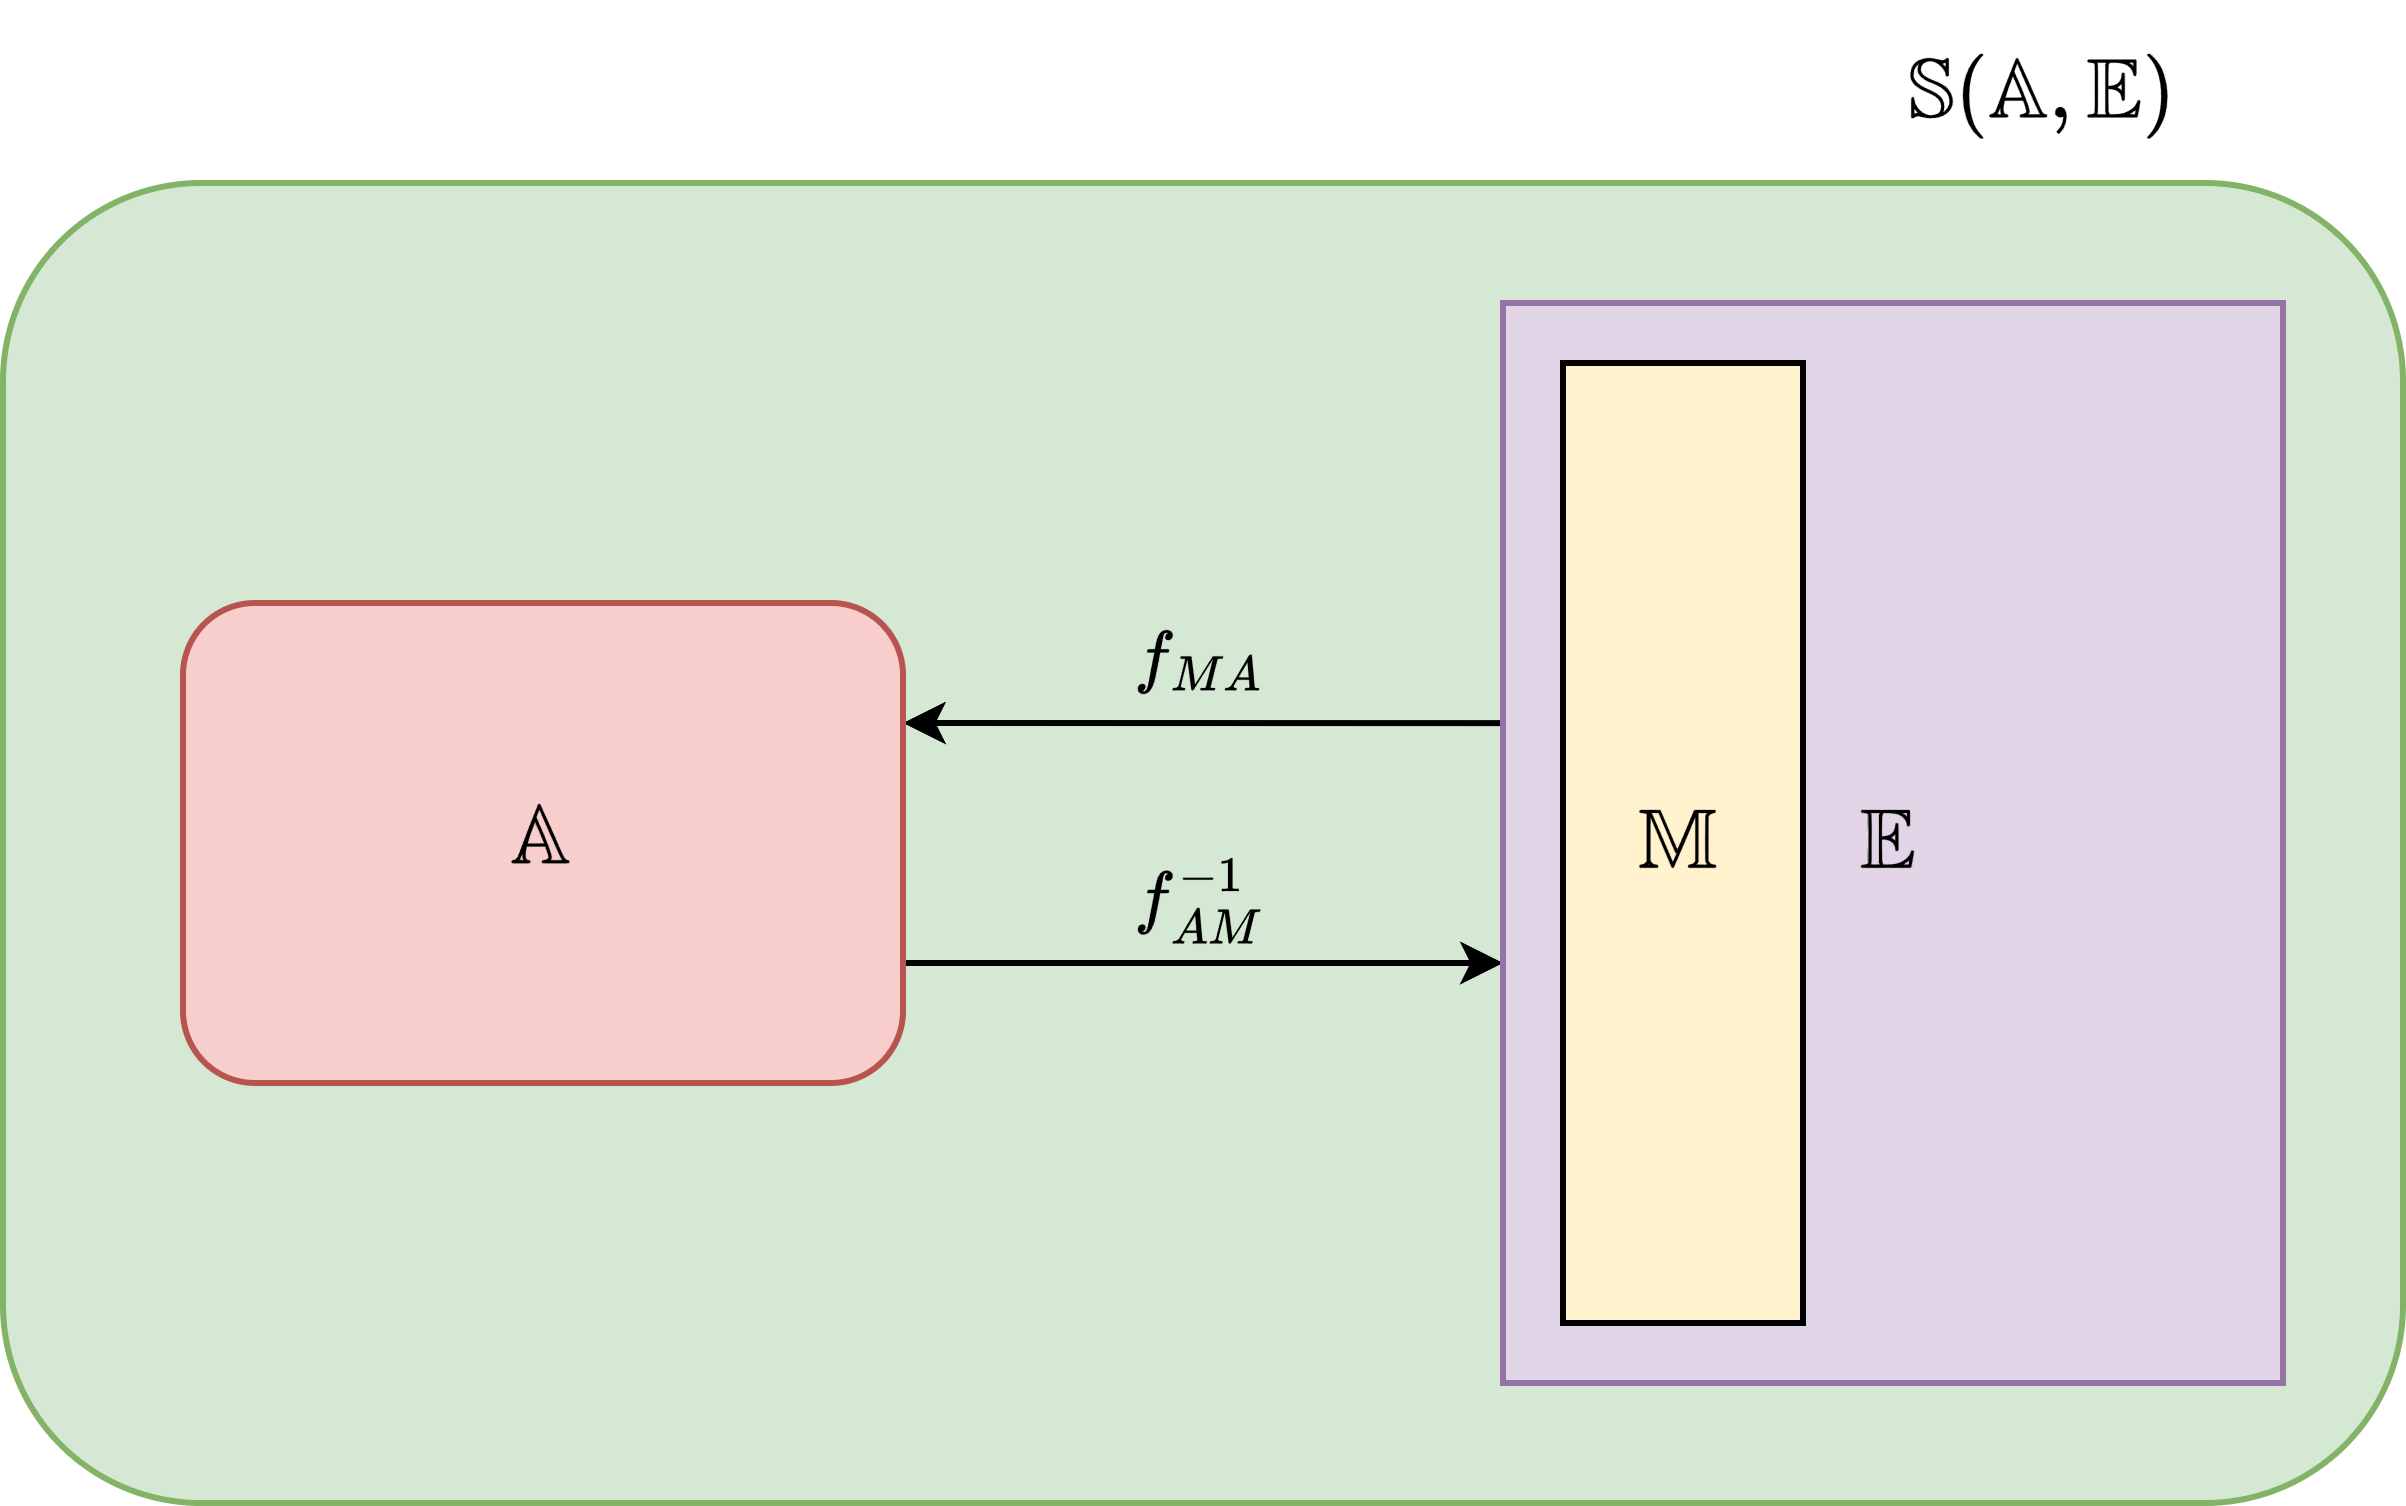
\includegraphics[width=0.5\textwidth]{img/model_representation.png}
  \caption{\textbf{Illustration of ambiance and encoding space, alongside a specific structural compact on the encoding}. The notation shifted to $\mathbb{A,M,E}$, but nevertheless represents the same structure. Here, as we can see, the system space contains ambiance and encoding space, alongside a specific encoding-related structure $\mathcal{M}$, and then two decoding and encoding which is short for interpreting between the two encoding spaces.}
\end{figure}

We understand this as inference of structures and objects into an interpretable and operational form. Specifying structures of certain objects, specifying properties of certain objects, the process of describing starting from static form, is inferred in the encoding sense. To encode objects, then in the ambiance space, require a representation framework that is powerful or rigid enough, to express particular properties and descriptions available to describe such object. We call it also the \textit{language} $\mathcal{L}_{E}$ of the encoding space, and subsequently, of the system space. 

The definition of the ambiance space is fairly arbitrary. What can be made of it to specify $\mathcal{A}$ more concretely? The space of objects has its own minimal language, we denote as $\mathcal{L}_{E}^{*}$. Taking inspiration from quantum physics, the ambiance space captures the \textit{state} of the system to a given particular \textit{state space}, the cardinality or size of the system in consideration, and object's structure of state space level. To clarify this, we can look both of the encoding of abstraction. An object $x$ has two type of general description - the overall $x$ state, lies in the state space $\mathcal{X}_{S}$, and the specific $x$-only description, the description space $\mathcal{X}_{D}$. These two spaces work alongside each other. For example, in the static case, $x$ has no variation, the state space and the description space is related such that there will be a description for specific state of $x$ in $\mathcal{X}_{S}$, and vice versa of a corresponding state. For a dynamic system, then, of any variation from $x_{1}\to x_{2}$ in the state space, then there exists a quantified variation that explains such variation in the state space. Conversely, if one wish to vary certain description of the description space, then there will have to exist a corresponding variation in the state space. This is a simple concept, but explains the relation between them. Coincidentally, the state space is described, within and of the ambiance space, and encoding space for the description space. 

Given the system $\mathcal{S}=(\mathcal{A},\mathcal{E}(\mathcal{L}_{E}))$ by then, There exists the encoding function, $f_{e}: \mathcal{A}\to \mathcal{E}(\mathcal{L}_{E})$ by functional notation. There also then exists the inverse mapping $f_{e}^{-1}$. These are called \textit{correspondence functions}, and we should know how to express them in later section of interest, when we start working on the construction of the learning theory on top. For now, though, the main function of them is to relate between the two spaces together, as 

\subsection{Groundwork of systems}

The system itself has some particular structures and working relations altogether, such as given by the definitions above. As we explained, the system itself contains two spaces copulated together. Let us examine it with an example. 

Let take a system $\mathcal{S}_{0}$. This system contains the ambiance space of response paradigm, for example, if in physics, the set of particles observations in specific potential landscape - for example, inside a potential well or not. Then, we have the ambiance space $\mathcal{A}=\{a_{i}\}^{n}$ of such particles. The minimal language here is the positional intrinsic space $(x,y,z,\dots)$. The reason why in this case we choose it is because it is intrinsic of the object by itself - the object exists in such space, instead of the object draws out such description by itself. The encoding space then, includes the language $\mathcal{L}_{E}$, with alphabet or description sets $\{p_{1},p_{2},\dots,\}$. In our case, then, the role of the language is to describe the object via the encoding space, and certain relation of it. 

A property $p_{i}\in \mathcal{E}$ is \textit{connected} (dependent) to the ambiance space $\mathcal{A}$, if for all taken expression of $p_{i}$ for any corresponding $x_{i}$, then $p_{i}$ is per definition, not of a constant quantity. If it is, then $p_{i}$ is unconnected (independent) of the system description. Such is for example, the mass $m$ of the particle at any given point is a static and constant quantity, but electric charge $q$ or something else, might depend on the configuration in the ambiance space for its quantification to take effect. Certain quantity depends on the evolution of $x_{i}$ over specified axis, usually time $t$, to be specified, for example, velocity, or displacement. Such are secondary quantity, and is harder to define. 

We can also remove and strip down everything to its most natural state in the ambiance space. That is, to make the object to be totally abstract as a singular existential state. It is similar to asking an apple to exist, with the only description now available is the cardinality of the object itself. And in such sense, we can then also use a fairly typical view of \textit{graph theory} to aid in such description. However, as said, we must be very careful when introducing new concepts of interpretations. 

These two languages, $\mathcal{L}^{*}$ and $\mathcal{L}_{E}$ are what called the \textit{configuration} of the system. Without it, the system itself cannot exist, because they form the basis of forming the model and the system the model lives and acts on. How can we relate them? For once, as we argued of the state space, the state of the system at large can be considered, strip to bare minimum, an \textit{object cardinality language}. 

\begin{definition}[Ambiance language]
  The language $\mathcal{L}^{*}$ of the ambiance space $\mathcal{A}$ of arbitrary size and shape, can be expressed minimally into the \textit{object cardinality class} (OCC) in which every object is specified by the pair $(i,y)$ for identifier $i$ and cardinality $y$. Hence, in general, the minimal OCC is the space $(I,\mathbb{N})$, for arbitrary identifier.
\end{definition}

At this point, an inquiry must be pointed at. The use of the word language in our formal treatment is not similar to the usual language typically seen in of mathematics and the like. It can be, or should be, referred to as the operational or representation language instead. Mathematically speaking, we can consider it a wrapper on the standard mathematical language. Thereby, a lot of components we use would be taken without proof or formalism required, out from the mathematical language itself. So what is it that we are actually using? These languages have the role to describe the system in certain manner only, within a scheme of quantization and an encoding method. For now, what we are discussing refers to the system without the \textit{model} in it. The goal later is then to exhibit that our models can indeed, work within such language interpretation. 

Finally, we would like to talk about the correspondence in actuality between the two space of the system space. Inherently in our expression, we specified that those two form the system space. However, we should also notice that this does not specifically specify how and what, for in the ambiance space, such object $o\in \mathcal{A}$ can be transitioned in side such space, given the description $\mathcal{L}^{*}$. For example, in the positional coordinate, what acts on the particle for its positional description to move from one point to another? Hence, we might as well consider the current system space as being treated in a static form, such that there exists no additional structure that governs such transition. If now there exists such structure, adding a dynamic encoding, and with a transiting structure, then we will call it a \textbf{dynamic system space}.

\subsection{Cardinality space}

It is fairly subjective, but well-needed partition. We have been speaking of the encoding space and ambiance for a while now, but there is a problem. We have subconsciously removed the aspect of the object not being encoded in the way that we actually entitled it to be in the same way. What is this? 

For starter, an object itself must exist. Of a system in consideration, entities within it has their own rules, their own structures, their own properties and behaviours that one then might take it as of its own, not quantized by experiments but intrinsic of itself, like volumes. Thereby. it would be lacking to presume every system to conform to the ambiance-encoding form, since sometimes what we only need is the existence specification of the system, and then the structure is encoded and governed, given a correct representation and encoding, of the encoding space. Thereby, it would be better to redefine what has been done above into a three-component system instead. Hence, we introduce the generalized system, with the following definition. 

\begin{definition}[Cardinality space]
  The cardinality space, denoted $\mathcal{C}$, is a 2-tuple $(I,\mathbb{N})^{n}$ where $I$ is the type of $n$ arbitrary objects, and $\mathbb{N}$ the cardinality of each type with respect to the $n$ set itself. 
\end{definition}

\begin{definition}[Ambiance space, formal definition]
  
\end{definition}


\begin{definition}[Encoding space, formal definition]
  
\end{definition}

In a sense, if we talk about a functional perspective, then $\mathcal{S}:(\mathcal{A}\to y)(\mathcal{E}\to x,f)(\mathcal{C}\to (I,\mathbb{N}))$ where $(I,\mathbb{N})$ is the cardinality of each type of category, suggested by $I$, together with the discrete number of them in natural number set. We assume the mathematical structure already defined of its foundation. 

\subsection{Probability}

Probability is a loose concept, most generally speaking. Usually, it refers to the uncertainty in our action, hence taken of virtue of subjectivity given certainty being not absolute. As reconciled by \cite{Nau2001_DeFinettiWasRight,deFinetti1990_TheoryProbability,Elliot2019_DeFinettiPhilosophy}, probability can be described to be of the \textit{degree of belief} of certain agent abstraction - an object or specimen that receives and act on the environment it beholds. In such sense, we can also interpret our system to explain the uncertainty that unfolds. 

Taken as an observer tasked with predicting and interpreting the system $\mathcal{S}_{0}$, then, by the standard definition of ambiance space. A system that is \textit{total predictable} and \textit{deterministic} if, the encoding space is empty, $\mathcal{E}=\varnothing$, and $\mathcal{L}^{*}=\mathcal{L}_{E}$. What this means is that all descriptions are known, the language is observable from such, and there are no encoding. This is the \textit{ideal system}. 

\section{The concept of learning}


